% =============================================================================
% CHAPITRE 5 — INTELLIGENCE ARTIFICIELLE ET DÉTECTION DES ANOMALIES
% =============================================================================

\chapter{Intelligence artificielle et détection des anomalies}

% =============================================================================
% 5.1 INTRODUCTION
% =============================================================================

\section{Introduction}

L'intelligence artificielle constitue l'un des éléments centraux de la
solution Droppy. Elle permet d'analyser automatiquement les données de
télémétrie afin d'identifier des comportements inhabituels et d'estimer
l'évolution future de la consommation.

L'approche retenue ne repose pas sur un unique mécanisme. Le service
d'intelligence artificielle combine des règles métier avec des méthodes
d'apprentissage automatique et de prévision. Cette combinaison permet
d'exploiter à la fois les connaissances liées au fonctionnement du réseau
et les comportements observés dans les données.

Le pipeline développé dans Droppy peut être résumé comme suit :

\begin{center}
\textbf{Données}
$\rightarrow$
\textbf{Nettoyage}
$\rightarrow$
\textbf{Prétraitement}
$\rightarrow$
\textbf{Détection}
$\rightarrow$
\textbf{Agrégation}
$\rightarrow$
\textbf{Résultat}
\end{center}


% =============================================================================
% 5.2 PIPELINE DE TRAITEMENT
% =============================================================================

\section{Pipeline de traitement des données}

Avant l'application des mécanismes de détection, les données sont chargées,
nettoyées puis préparées pour les différents traitements.

Le microservice IA sépare cette chaîne en plusieurs étapes correspondant au
chargement des mesures, au nettoyage et au prétraitement des données. Cette
organisation permet de disposer d'un flux de traitement homogène avant
l'exécution des différents mécanismes d'analyse.

\begin{figure}[H]
    \centering
    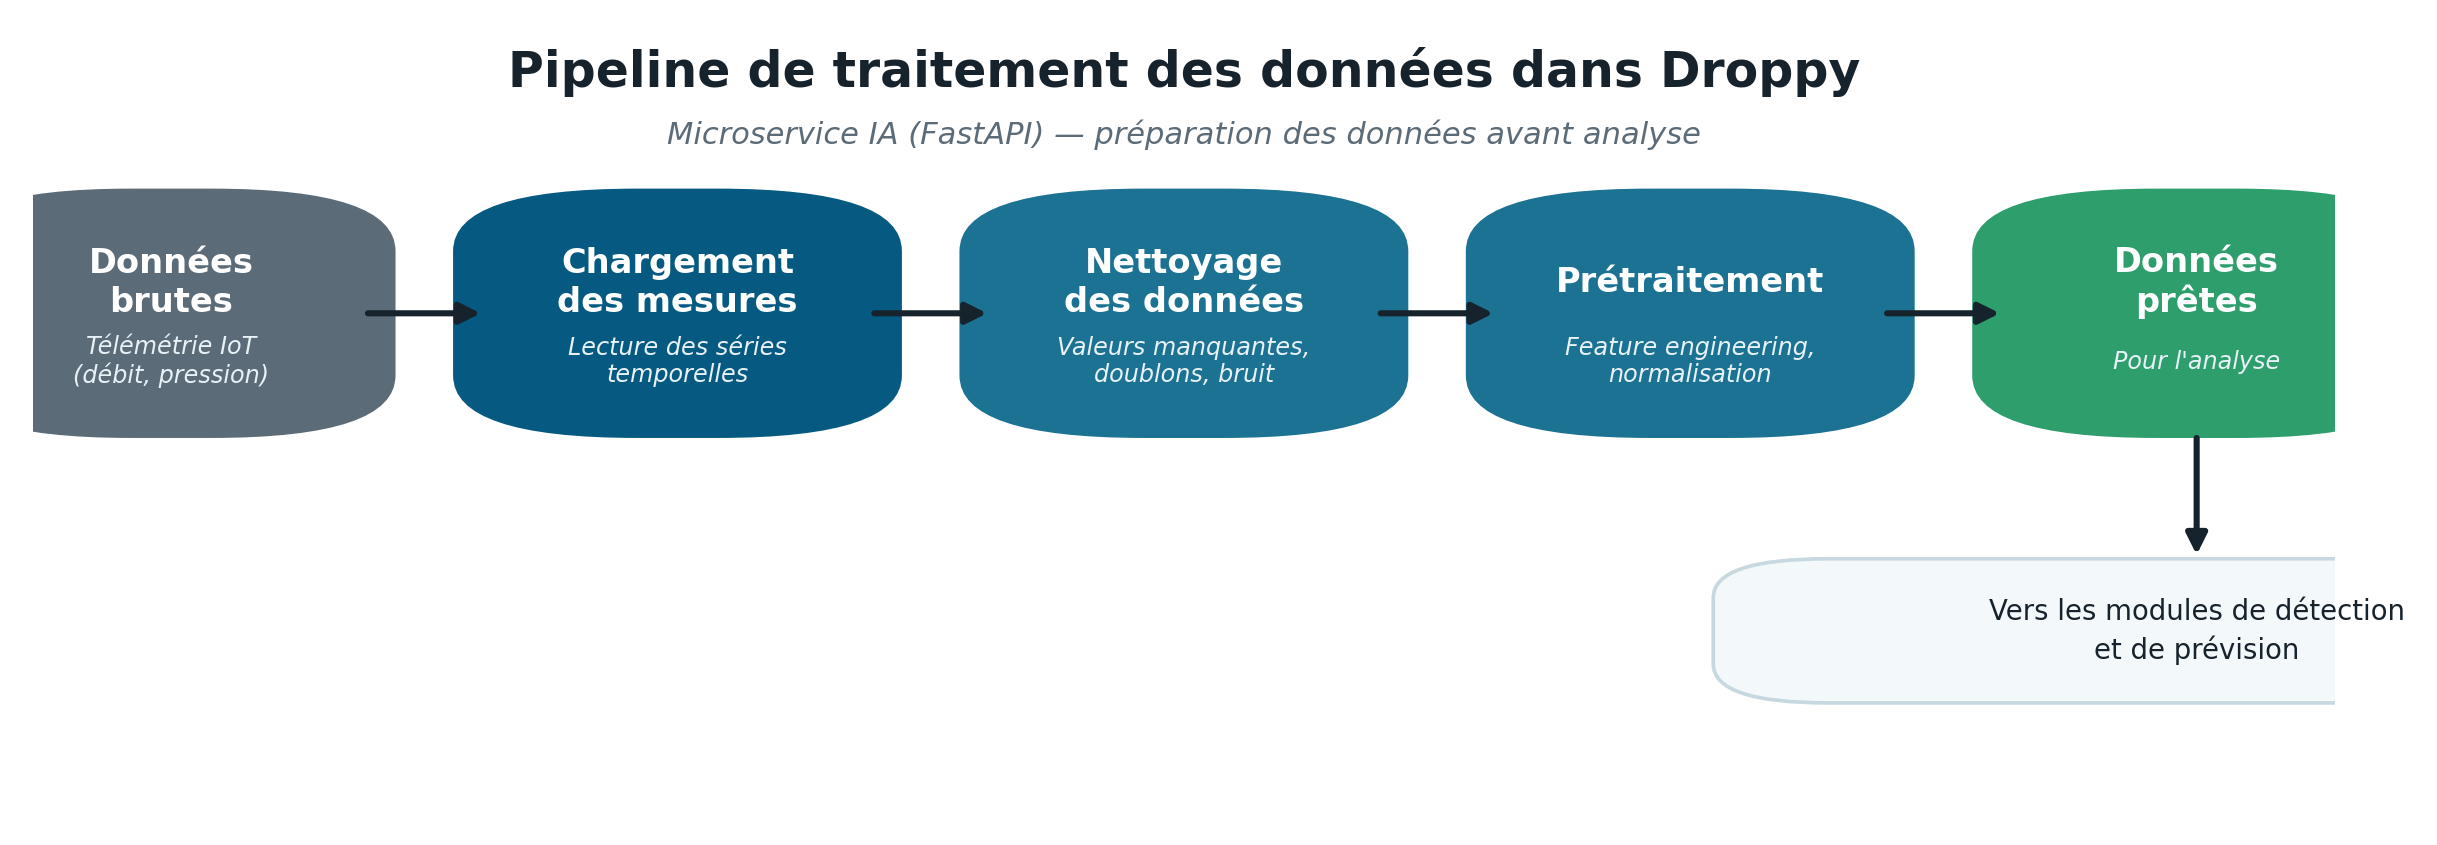
\includegraphics[width=0.90\textwidth]{images/pipeline-ia.png}
    \caption{Pipeline de traitement des données dans Droppy}
    \label{fig:pipeline-ia}
\end{figure}

Cette séparation permet également de réutiliser les mêmes étapes de
préparation pour les différents mécanismes d'analyse.


% =============================================================================
% 5.3 STRATÉGIE DE DÉTECTION
% =============================================================================

\section{Stratégie de détection des anomalies}

La détection mise en œuvre dans Droppy repose sur une approche hybride.
Lorsqu'une prédiction est demandée, le microservice exécute plusieurs
mécanismes indépendants puis regroupe leurs résultats.

Quatre sources de détection sont actuellement intégrées :

\begin{itemize}

    \item la détection du \textit{Minimum Night Flow} ;

    \item la détection d'incohérences liées aux vannes ;

    \item la détection statistique par \textit{Isolation Forest} ;

    \item la détection d'écarts de consommation à partir du modèle de
    prévision.

\end{itemize}

Les résultats sont ensuite regroupés et les événements correspondant au même
type et au même intervalle temporel sont dédoublonnés.

\begin{figure}[H]
    \centering
    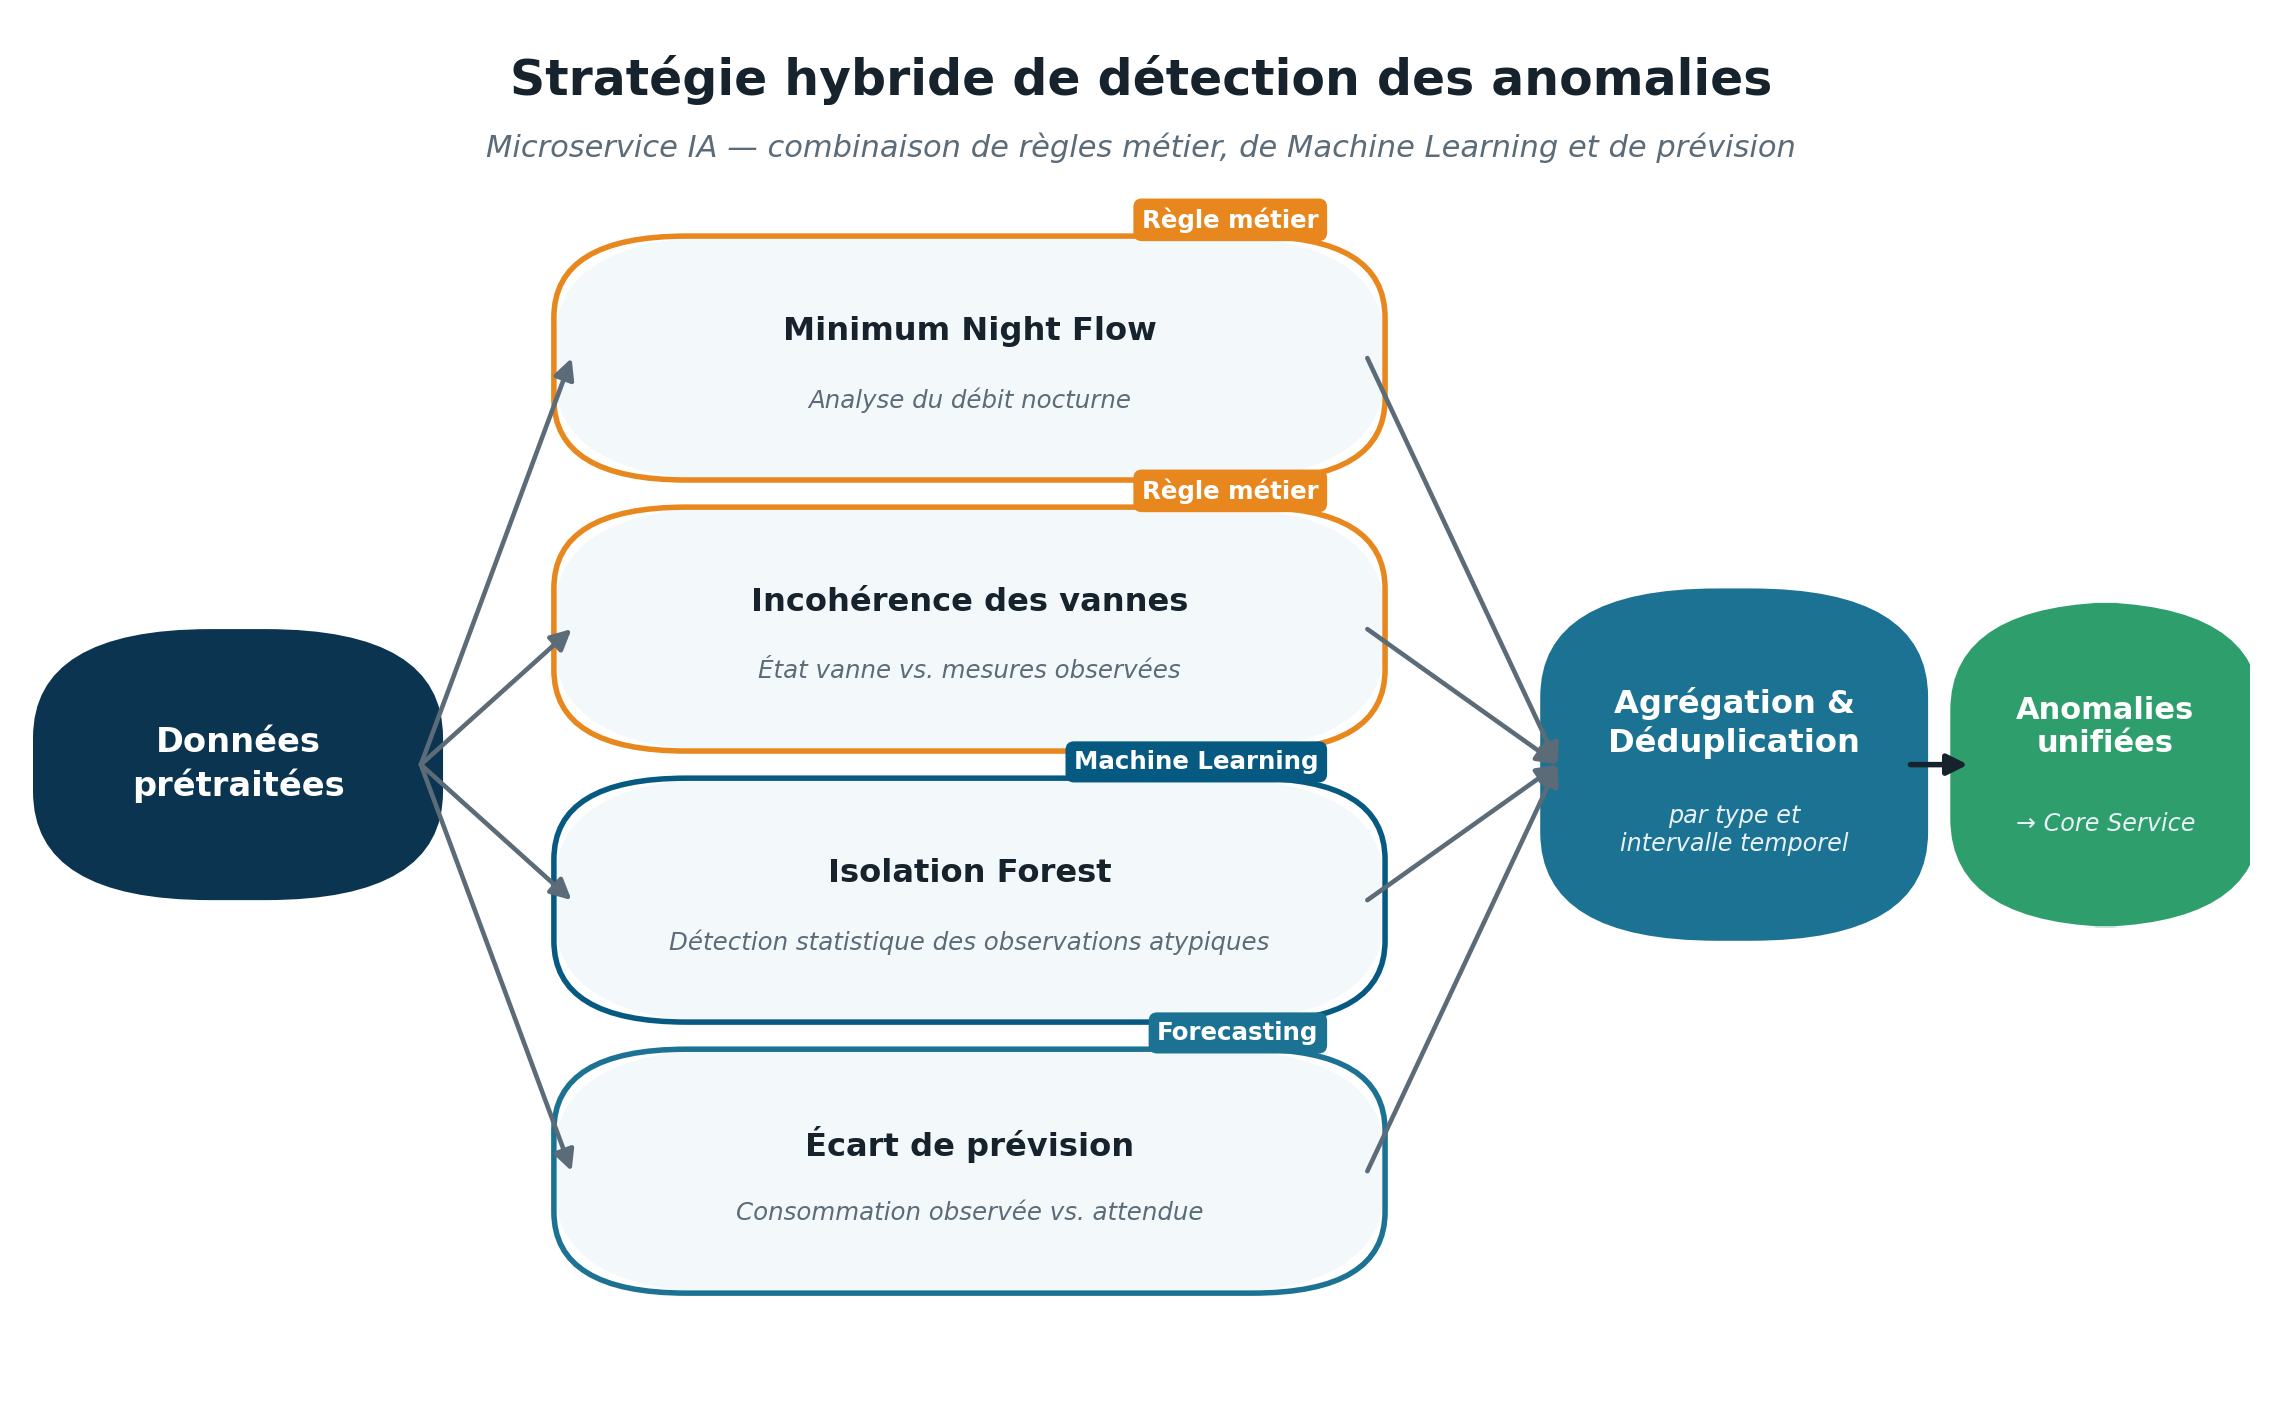
\includegraphics[width=0.90\textwidth]{images/strategie-detection.png}
    \caption{Stratégie hybride de détection des anomalies}
    \label{fig:strategie-detection}
\end{figure}


% =============================================================================
% 5.4 DÉTECTION PAR RÈGLES MÉTIER
% =============================================================================

\section{Détection basée sur les règles métier}

\subsection{Minimum Night Flow}

Le premier mécanisme repose sur l'analyse du débit pendant les périodes
nocturnes. L'objectif est d'identifier des situations dans lesquelles le
comportement observé s'écarte du fonctionnement attendu pendant ces
périodes.

Cette approche permet d'intégrer directement une connaissance métier dans
le processus de détection, sans dépendre exclusivement d'un modèle
d'apprentissage automatique.

\subsection{Incohérence liée aux vannes}

Le second mécanisme recherche des incohérences entre l'état d'une vanne et
le comportement observé dans les mesures.

Cette règle permet de détecter des situations dans lesquelles les mesures
observées ne correspondent pas au fonctionnement attendu du dispositif.


% =============================================================================
% 5.5 DÉTECTION PAR ISOLATION FOREST
% =============================================================================

\section{Détection par Isolation Forest}

En complément des règles métier, Droppy utilise l'algorithme
\textit{Isolation Forest} pour identifier automatiquement les observations
qui présentent un comportement inhabituel.

Contrairement à une classification supervisée classique, cette méthode est
adaptée à la détection d'observations atypiques. Le modèle est entraîné à
partir des données préparées puis utilisé lors de l'analyse d'un dispositif.

Dans l'implémentation de Droppy, le modèle est chargé pour le dispositif
concerné et appliqué aux données prétraitées. Le résultat produit contribue
ensuite à la liste globale des anomalies.

\begin{figure}[H]
    \centering
    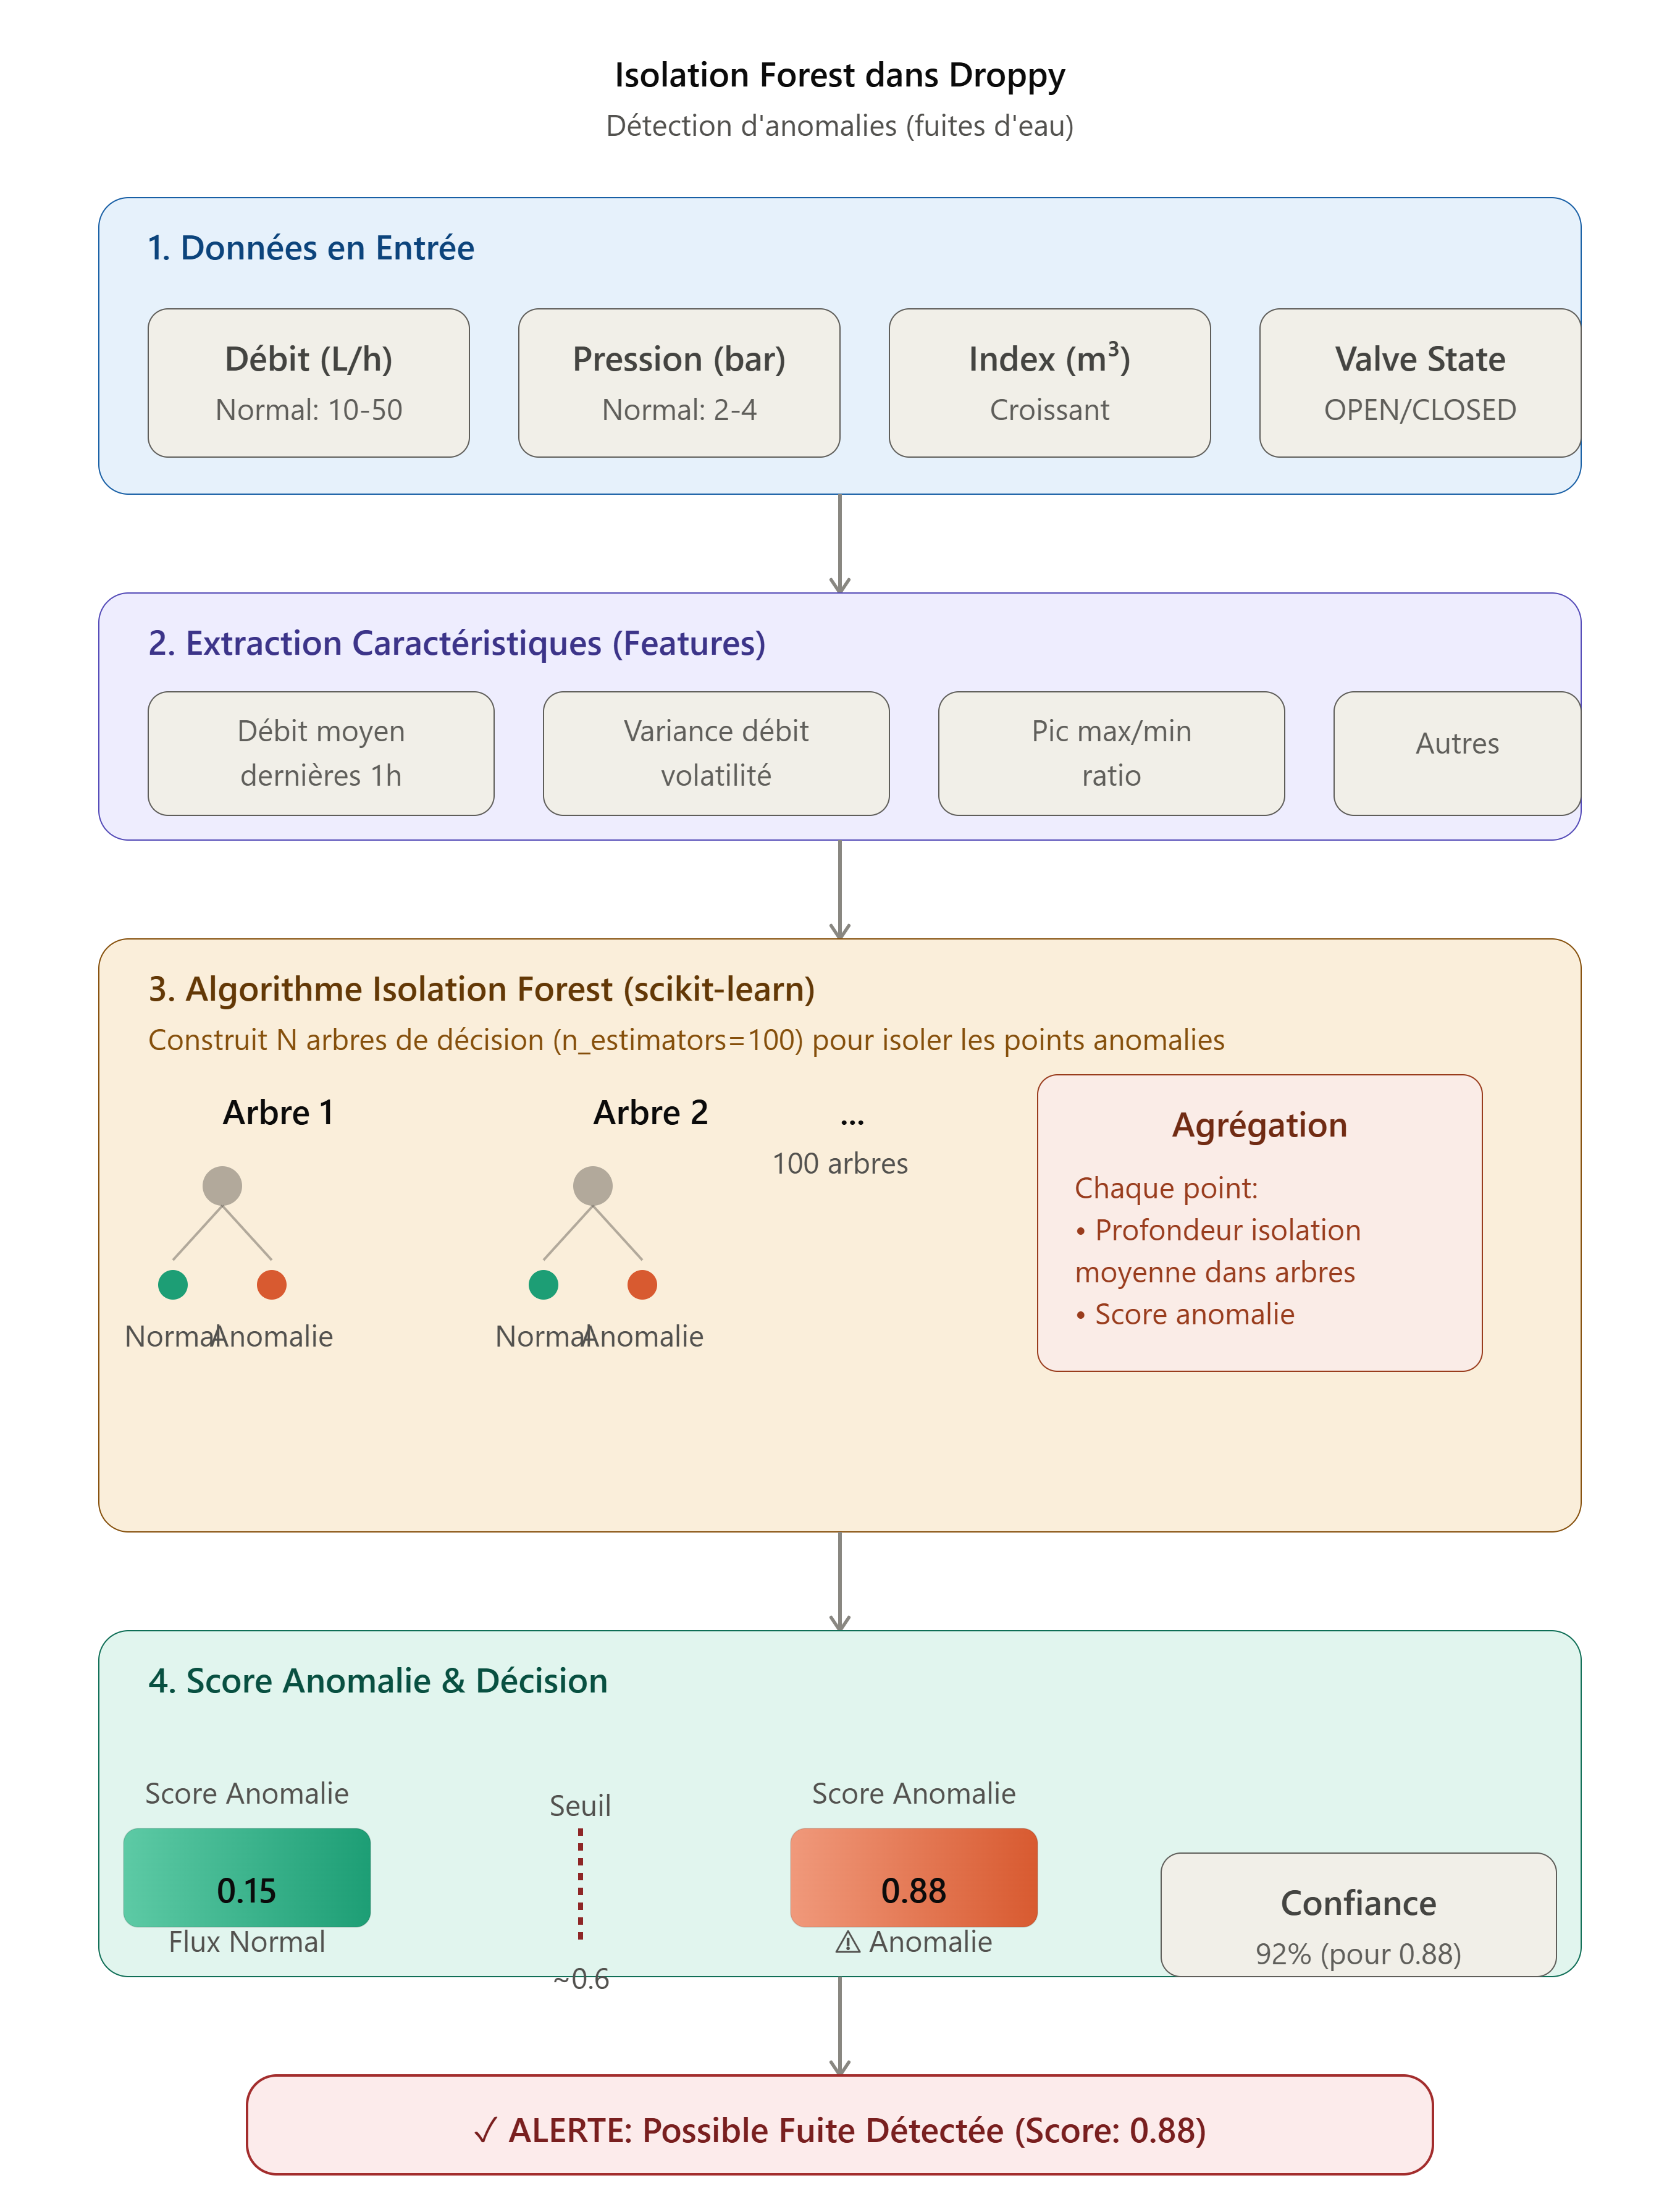
\includegraphics[width=0.85\textwidth]{images/isolation_forest_droppy_principle.png}
    \caption{Principe d'utilisation de l'Isolation Forest dans Droppy}
    \label{fig:isolation-forest}
\end{figure}


% =============================================================================
% 5.6 PRÉVISION DE CONSOMMATION
% =============================================================================

\section{Agrégation des résultats}

L'une des caractéristiques importantes de l'approche adoptée est la
combinaison des différentes sources de détection.

Pour une même période d'analyse, les résultats issus des règles métier,
de l'Isolation Forest et de l'analyse de déviation de consommation sont
regroupés dans une même réponse.

Le système applique ensuite une étape de déduplication afin d'éviter de
retourner plusieurs fois un même événement lorsqu'il est identifié par
plusieurs mécanismes.

Cette stratégie permet de produire une sortie unifiée destinée au Core
Service et, finalement, au dashboard Droppy.


% =============================================================================
% 5.9 RÉSULTAT DE L'ANALYSE
% =============================================================================

\section{Résultat de l'analyse}

Chaque anomalie produite par le microservice contient plusieurs informations
permettant son exploitation par les composants du système.

Le résultat de prédiction comprend notamment :

\begin{itemize}

    \item le type de l'anomalie ;

    \item le score associé à la détection ;

    \item l'intervalle temporel concerné ;

    \item le niveau de sévérité.

\end{itemize}

Ces informations sont ensuite transmises au Core Service afin d'être
intégrées dans le système de supervision.


% =============================================================================
% 5.10 API DU SERVICE INTELLIGENT
% =============================================================================

\section{Exposition des fonctionnalités IA}

Les fonctionnalités d'intelligence artificielle sont exposées à travers le
microservice FastAPI.

Trois opérations principales sont proposées :

\begin{itemize}

    \item \texttt{/train/\{mac\}} : entraînement ou réentraînement des
    modèles associés à un dispositif ;

    \item \texttt{/predict/\{mac\}} : exécution de la détection combinant
    les différents mécanismes d'analyse ;

    \item \texttt{/forecast/\{mac\}} : génération des prévisions de
    consommation.

\end{itemize}

Cette séparation permet au Core Service de solliciter indépendamment les
opérations d'entraînement, de détection et de prévision.


% =============================================================================
% 5.11 SYNTHÈSE
% =============================================================================

\section{Synthèse}

L'intelligence de Droppy repose ainsi sur une combinaison de plusieurs
mécanismes complémentaires.

Les règles métier permettent d'intégrer les connaissances liées au
fonctionnement du réseau, tandis que l'Isolation Forest apporte une capacité
de détection automatique des comportements atypiques. Le modèle de prévision
complète cette approche en permettant à la fois d'estimer la consommation
future et d'identifier des écarts par rapport au comportement attendu.

Cette approche hybride constitue le cœur analytique de Droppy et permet de
transformer les données de télémétrie en événements exploitables par la
plateforme de supervision.


% =============================================================================
% 5.12 CONCLUSION
% =============================================================================

\section{Conclusion}

Ce chapitre a présenté le fonctionnement de la composante d'intelligence
artificielle de Droppy.

La solution combine un pipeline de préparation des données, des règles
métier, l'algorithme Isolation Forest et un mécanisme de prévision de
consommation. Les résultats issus de ces différents traitements sont
agrégés afin de produire une vision unifiée des anomalies détectées.

Le chapitre suivant sera consacré aux tests et à la validation de la solution
afin d'évaluer le comportement des différents composants et les résultats
obtenus.